% \documentclass[oneside]{report}
\documentclass[oneside,final,14pt,a4paper]{extreport}
\usepackage[T2A]{fontenc}

\usepackage{vmargin}
\setpapersize{A4}
\setmarginsrb{2.5cm}{2cm}{2cm}{2cm}{0pt}{10mm}{0pt}{13mm}
\usepackage{setspace}
\sloppy
\setstretch{1.5}
\usepackage{indentfirst}
\parindent=1.25cm

%%%%% ADDED TO SUPPORT TT BOLD FACES %%%%
\DeclareFontShape{OT1}{cmtt}{bx}{n}{<5><6><7><8><9><10><10.95><12><14.4><17.28><20.74><24.88>cmttb10}{}
\renewcommand{\ttdefault}{pcr}
%%%%% END %%%%%%%%%%%%%%%%%%%%%%%%%%%%%%% 
\usepackage{atbegshi,picture}
\AtBeginShipout{\AtBeginShipoutUpperLeft{%
  \put(\dimexpr\paperwidth-1cm\relax,-1.5cm){\makebox[0pt][r]{
\includegraphics[width=3cm]{figs/inno}}}%
}}


\usepackage[english]{babel}
\usepackage[backend=biber,style=ieee,autocite=inline]{biblatex}
\bibliography{ref.bib}
\DefineBibliographyStrings{english}{%
  bibliography = {References},}
\usepackage{blindtext}
\usepackage{pdfpages}
\newenvironment{bottompar}{\par\vspace*{\fill}}{\clearpage}
\usepackage{amsmath,amsfonts}

\usepackage{amsthm}
\newtheorem{theorem}{Theorem}
\newtheorem{corollary}{Corollary}
\newtheorem{lemma}{Lemma}
\newtheorem{proposition}{Proposition}
\theoremstyle{definition}
\newtheorem{definition}{Definition}
\theoremstyle{remark}
\newtheorem*{remark}{Remark}
\theoremstyle{remark}
\newtheorem*{example}{Example}



\usepackage{float}
\usepackage{graphicx}
\graphicspath{{figs/}} %path to images
\usepackage{array}
\usepackage{multirow,array}
\usepackage{caption}
\usepackage{subcaption}
\usepackage{hyperref}
\usepackage{paralist}
\usepackage{listings}
\usepackage{zed-csp}
\usepackage{fancyhdr}
\usepackage{csquotes}
\usepackage{color}

\usepackage{upgreek} 
\usepackage{bm}
\usepackage{hyperref}
\usepackage{setspace}
\usepackage{booktabs}
\usepackage{multirow}
\usepackage{longtable}
\usepackage[font=singlespacing, labelfont=bf]{caption}

%Hints
\newcommand\pic[1]{(Fig. \ref{#1})} %Ref on figure
\newcommand\tab[1]{(Tab. \ref{#1})} %Ref on table


\usepackage{enumitem}
\newlist{inlinelist}{enumerate*}{1}
\setlist*[inlinelist,1]{%
  label=(\arabic*),
}




\pagestyle{fancyplain}

% remember section title
\renewcommand{\chaptermark}[1]%
	{\markboth{\chaptername~\thechapter~--~#1}{}}

% subsection number and title
\renewcommand{\sectionmark}[1]%
	{\markright{\thesection\ #1}}

\rhead[\fancyplain{}{\bf\leftmark}]%
      {\fancyplain{}{\bf\thepage}}
\lhead[\fancyplain{}{\bf\thepage}]%
      {\fancyplain{}{\bf\rightmark}}
\cfoot{} %bfseries


\newcommand{\dedication}[1]
   {\thispagestyle{empty}
     
   \begin{flushleft}\raggedleft #1\end{flushleft}
}

\begin{document}

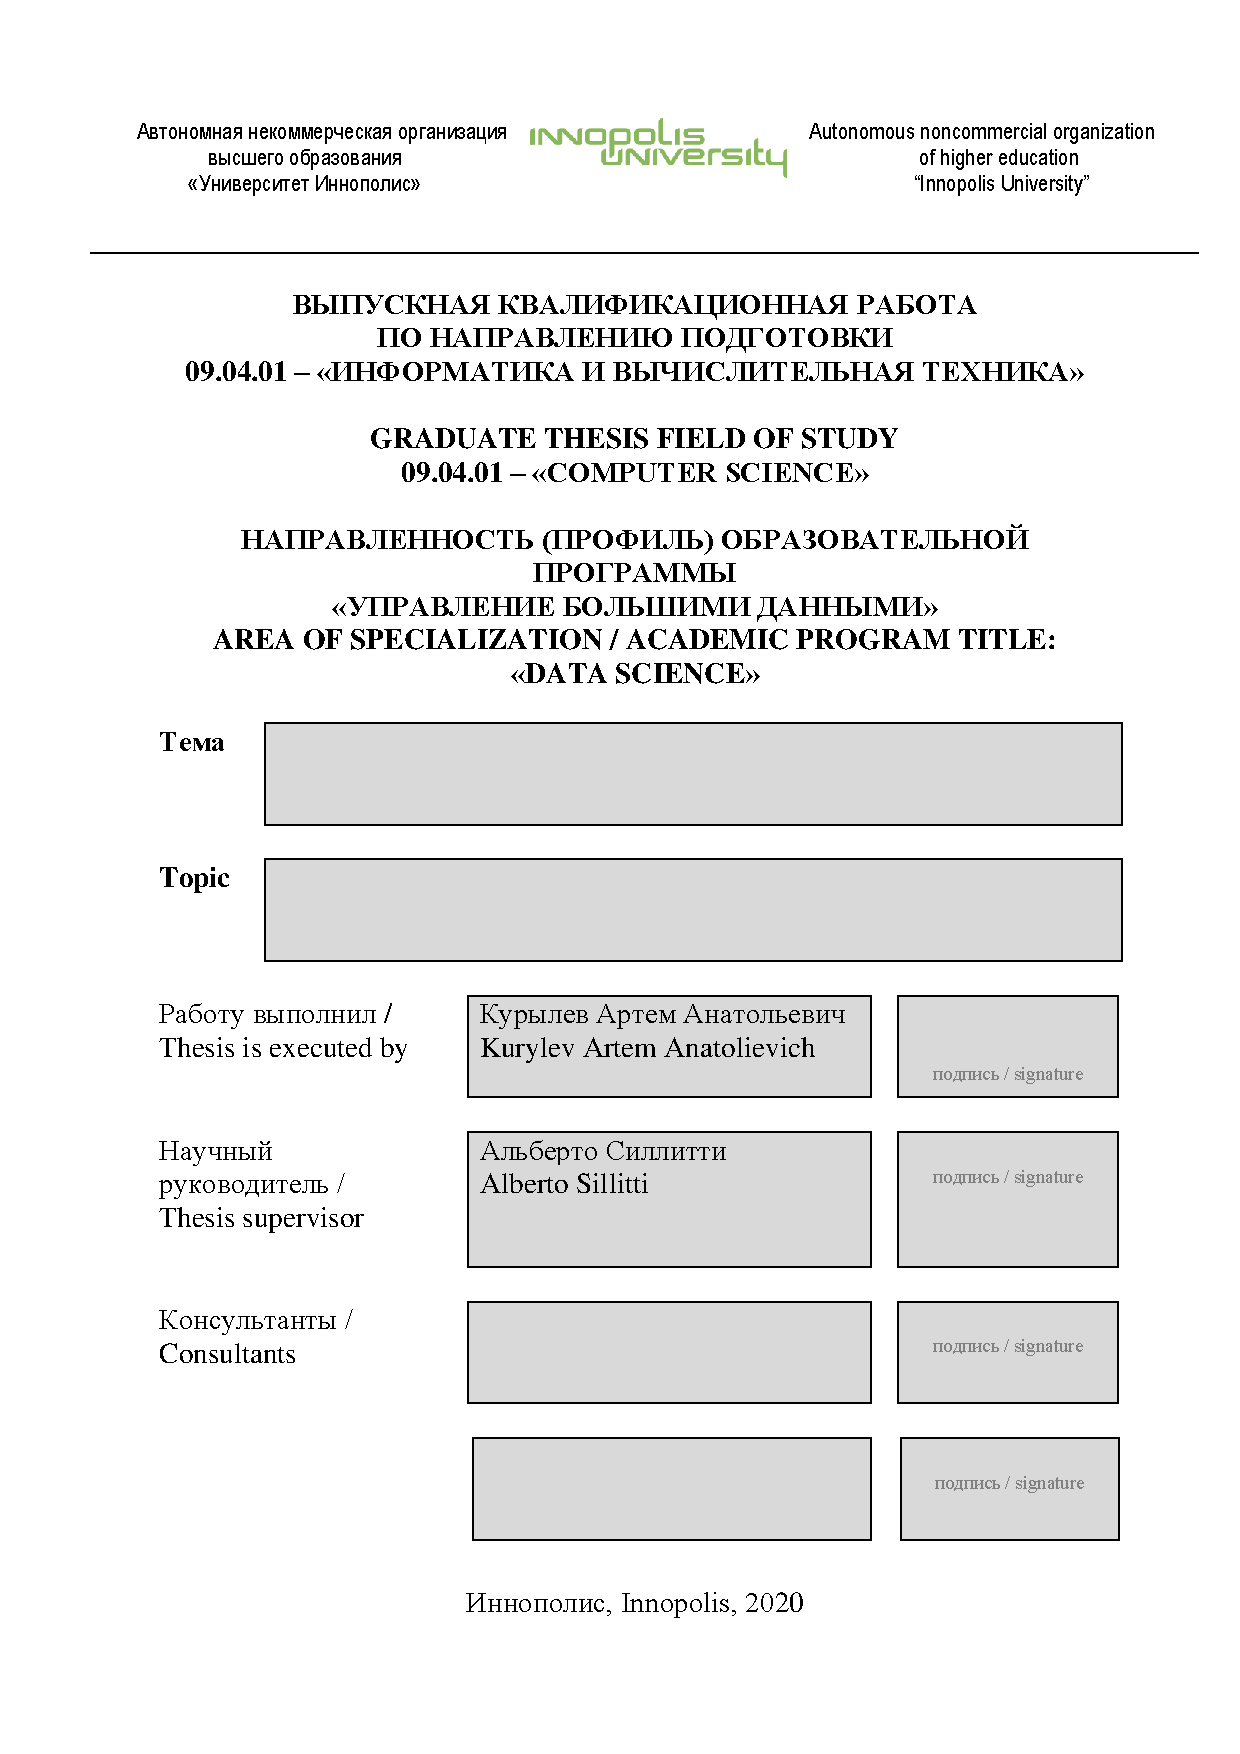
\includepdf[pages=-]{title.pdf}
\tableofcontents
\listoftables
\listoffigures


\newpage
\begin{abstract}
abstract \ldots
\end{abstract}
% Depend on above part
\setcounter{page}{6}
\chapter{Introduction}
\label{chap:intro}
\chaptermark{Optional running chapter heading}
\section{Spacing \& Type}
\label{sec:section}

This is a section. This is a citation without brackets. and this is one with brackets \cite{A}. Multiple \cite{A,B,C} Here's a reference to a subsection: \ref{sec:subsection}. The body of the text and abstract must be double-spaced except for footnotes or long quotations. Fonts such as Times Roman, Bookman, New Century Schoolbook, Garamond, Palatine, and Courier are acceptable and commonly found on most computers. The same type must be used throughout the body of the text. The font size must be 10 point or larger and footnotes\footnote{This is a footnote.} must be two sizes smaller than the text\footnote{This is another footnote.} but no smaller than eight points. Chapter, section, or other headings should be of a consistent font and size throughout the ETD, as should labels for illustrations, charts, and figures.  

\subsection{Creating a Subsection}
\label{sec:subsection}

\subsubsection{Creating a Subsubsection}

\paragraph{This is a heading level below subsubsection}

And this is a quote: 
%
\begin{quote}
\blindtext
\end{quote}

This is a table:
% currsize is not set in the long table environment, so we need to set it before we set it up.
\makeatletter
\let\@currsize\normalsize
\makeatother

% tabular environments are set to be single-spaced in the  thesis class,  but long tables do not use tabular
% to get around this, set the spacing to single spacing at the start of the long table environment, and set it back to double-spacing at the end of it

\begin{longtable}{cc}
\caption[This is the title I want to appear in the List of Tables]{This is a caption.} \label{tab:pfams} \\
\hline
A & B \\
\hline
\endfirsthead
\multicolumn{2}{@{}l}{\textbf{Table \thetable} \ldots continued} \\
\hline
A & B \\
\hline
\endhead
a1 & b1 \\
a2 & b2 \\
a3 & b3 \\
a4 & b4 \\
\hline
\end{longtable}


The package ``upgreek'' allows us to use non-italicized lower-case greek letters. See for yourself: $\upbeta$, $\bm\upbeta$, $\beta$, $\bm\beta$. Next is a numbered equation:
\begin{align}
\label{eq:name}
\|\bm{X}\|_{2,1}={\underbrace{\sum_{j=1}^nf_j(\bm{X})}_{\text{convex}}}=\sum_{j=1}^n\|\bm{X}_{.,j}\|_2
\end{align}
The reference to equation (\ref{eq:name}) is clickable. 
\section[Theorems, Corollaries, Lemmas, Proofs, Remarks, Definitions and Examples]{Theorems, Corollaries, Lemmas, Proofs, Remarks, Definitions,and Examples}

\begin{theorem}
\label{thm:onlytheorem}
\blindtext
\end{theorem}

\begin{proof}
I'm a (very short) proof.
\end{proof}

\begin{lemma}
I'm a lemma.
\end{lemma}

\begin{corollary}
I include a reference to Thm. \ref{thm:onlytheorem}.
\end{corollary}

\begin{proposition}
I'm a proposition.
\end{proposition}

\begin{remark}
I'm a remark. 
\end{remark}

\begin{definition}
I'm a definition. I'm a definition. I'm a definition. I'm a definition. I'm a definition. I'm a definition. I'm a definition. I'm a definition. I'm a definition. I'm a definition. I'm a definition. 
\end{definition}

\begin{example}
I'm an example.
\end{example}


\section[Optional table of contents heading]{Section with\\ linebreaks in\\the
name}


\Blindtext[2]





\chapter{Literature Review}
\label{chap:lr}
\chaptermark{Second Chapter Heading}



\section{Sources and methods of searching}
For the purposes of search of the articles I used three main sources: 
\begin{enumerate}
    \item ACM DIGITAL LIBRARY
    \item Google Scholar
    \item Springer Link
\end{enumerate}

\section{Comprehensive report}
In this section I will provide report for the articles I found in resources.
\begin{enumerate}
    \item \textbf{Deep Multi-Camera People Detection}
    
    \begin{enumerate}
        \item \textbf{Problem}
        
        In article \cite{chavdarova2017deep} authors stated addressed the problem of multi-view occupancy map estimation.
        \item \textbf{Method}
        
        They used two stages: Firstly they used to train CNN on dataset with monocular view and then retain d of its layers, that results in some embedding  \[\mathit{\psi:} \mathit{I} \rightarrow \mathit{R^Q}\] where Q is number of output layer in dth layer. Then concatenation of C these embeddings is a multi-view embedding \[\psi: \mathit{I^C}\rightarrow R^{CQ}\]and on top of that embeddings binary classifier was trained. And finally, Non maxima suppression(NMS) algorithm was applied to select most appropriate candidates.
        
        \item \textbf{Conclusion}
        
        Authors proposed end-to-end deep learning  method for multi=view people detection, which outperforms state-of-the-art models of that time.
        \item \textbf{Performance}
        
        Authors used the following metrics for evaluating performance of the model: MODA (Multiple Object Detection Accuracy), MODP (Multiple object detection precision) Precision and Recall. Their best Results are presented in the table \ref{tab:deep}
        \\
        
        \begin{center}
            \begin{longtable}{cc}
            \label{tab:deep} \\
            \hline
            Metric & Value\\
            \hline
            MODA & 0.94 \\
            \hline
            MODP & 0.68 \\
            \hline
            Precision & 0.98 \\
            \hline
            Recall & 0.97 \\
            \hline
            \caption[Metrics table for Deep Multi-Camera people detection]{Performance Metric} 
            \end{longtable}
            
        \end{center}
        
        \item \textbf{Strong Points}
        
        For the multiple views architecture of network presented in the article allows to parallelize computations. Authors also showed via their experiments that depth of the CNN as the feature extractor does not impact much on the result, so it allows to use shallower architectures.
        
        \item \textbf{Weak Points}
        
        The weakest point of the study is that even in PETS dataset, that was used for training and evaluating result, data was composed only from 8 views, that produces uncertainty about behavior of such system in case of using more views.
    \end{enumerate}
    \item \textbf{Monitoring Pedestrian Flow on Campus with Multiple Cameras using Computer Vision and Deep Learning Techniques}
    \begin{enumerate}
        \item \textbf{Problem}
        In article \cite{monitoring2019} Authors stated problem of milticamera person re-identification and tracking across non-overlapping cameras
        \item \textbf{Method}
        Authors adopted Part-Based Convolution Baseline (PCB) \cite{sun2017models}. Idea of this method is about dividing received from backbone tensor into sub regions, where each sub region represents some part of body. Authors of the article proposed special weighted loss, which is calculated as following \[\dfrac{\sum_{i=1}^p (w_i*l_i)}{\sum_{i=1}^p w_i} \] where $w_i$ corresponds to weight of each body part. They used DukeMTMC-reID\cite{zheng2017unlabeled} dataset for training and evaluating results.
        \item \textbf{Conclusion}
        Authors outperformed existing methods in Re-Identification task, and invented new weight loss adoption for the PCB approach. 
        \item \textbf{Performance}
        For evaluating Performance authors used two metrics - Rank-1 Accuracy and Mean Average precision(mAP). They are presented in the table \ref{tab:monitoringflow}
        \\
        
        \begin{center}
            \begin{longtable}{cc}
            \label{tab:monitoringflow} \\
            \hline
            Metric & Value\\
            \hline
            Rank-1 Accuracy(\%) & 84.0 \\
            \hline
            mAP(\%) & 71.6 \\
            \hline
            \caption[Metrics table for Monitoring Pedestrian Flow]{Performance Metrics} 
            \end{longtable}
            
        \end{center}
        
        \item \textbf{Strong points}
        Authors outperforms current state-of the art results in person identification task 
        \item \textbf{Weak points}
        Images from cameras include image from only one person and for the task of counting people there is need to have possibility to count multiple people from the single camera.
    \end{enumerate}
    \item \textbf{Locate, Size and Count: Accurately Resolving People in Dense Crowds via Detection}
    \begin{enumerate}
        \item \textbf{Problem}
        Authors in \cite{sam2019locate} stated the problem of dense crowd people counting.
        \item \textbf{Method}
        Authors introduced new architecture LCS-CNN, which consists of three modules. First is feature extractor at multiple resolutions, second is Top Feature Modulator, where information from features is fused, and then predictions on bounding boxes are made, and the third one is NMS, where valid candidates are selected. For the training of the model last part was replaced by GWTA Loss module, which includes pixel wise information.   
        \item \textbf{Conclusion}
        Authors outperformed existing state-of-the art methods for people crowd counting, and introduced new specific method exactly for people crowd counting, especially for the dense ones.
        \item \textbf{Performance}
        Authors presented two metrics for evaluating results of their model: MAE and MSE on two datasets - ShanghaiTech(ST) Part A \cite{7780439} and UCF-QNRF dataset \cite{idrees2018composition}. They are presented in the table \ref{tab:locatesizecount}
        \\ \\
        
        \begin{center}
            \begin{longtable}{cccc}
            \label{tab:locatesizecount} \\
            \hline
            MAE on ST part A &  MSE on ST part A & MAE on UCF & MSE on UCF\\
            \hline
            66.4 & 117.0 & 120.5 & 218.3 \\
            \hline
            \caption[Metrics table for Locate Size and Count in dense crowds]{Performance Metrics} 
            \end{longtable}
        \end{center}
        
        \item \textbf{Strong points}
        Accurate predictions in counting people in dense crowd, which is important if we use to use such a system in a malls or another big buildings, where a lot of people can be vied from single camera. Also time of inference is reasonable, that can be used in streaming data.
        \item \textbf{Weak points}
        Model used data only from single camera
    \end{enumerate}
    \item \textbf{DecideNet: Counting Varying Density Crowds Through Attention Guided Detection and Density Estimation}
    \begin{enumerate}
        \item \textbf{Problem}
        Authors in \cite{liu2017decidenet} stated problem of crowd counting in both low density and not low density areas. They represent this problem as a density map estimation 
        \item \textbf{Method}
        First authors generated density map, using Gaussian kernel for ground truth head positions. Architecture consists of 3 parts - RegNet, which is nothing else but a CNN with 5 convolution, DetNet which is built upon R-CNN network, and Quality Net that get as input two density maps from first two blocks and original image. After forwarding through this part all three density maps are concatenated and then jointed into one with Hadamard product. Loss function is calculated for each of the parts with using of ground truth map 
        \item \textbf{Conclusion}
        Authors created new model for crowd density estimation with combining both approaches for crowd density estimation - regression and detection. 
        \item \textbf{Performance}
        Authors evaluated their framework with two metrics - MSE and MAE on three datasets - Mall dataset \cite{chen2012mall}, ST part B \cite{7780439} and WorldExpo’10 dataset \cite{Zhang_2015_CVPR} 
        Results are presented in the table \ref{tab:decidenet}
        \begin{center}
            \begin{longtable}{ccc}
            \label{tab:decidenet} \\
            \hline
            Dataset & MAE &  MSE\\
            \hline
            ST part B & 1.52 & 1.9 \\
            Mall & 20.75 & 29.42\\
            WorldExpo & 9.23 & \\
            \hline
            \caption[Metrics table for DecideNet]{Performance Metrics} 
            \end{longtable}
        \end{center}
        
        \item \textbf{Strong points}
        Accurate results on different datasets, using combination of two different approaches for the task of crowd counting
        \item \textbf{Weak points}
        Architecture was tested on ST part B which is more sparse than part A. Architecture is using only one camera
    \end{enumerate}
    \item \textbf{A Reliable People Counting System via Multiple Cameras }
    \begin{enumerate}
        \item \textbf{Problem}
        In the article \cite{10.1145/2089094.2089107} authors stated the problem of counting people using multiple cameras. 
        \item \textbf{Method}
        Authors proposed architectures which consists of multilevel HOG and LBP descriptors. After this stages PCA and SVM were applied to created features and  candidates to select ones that are more likely to be actual persons
        \item \textbf{Conclusion}
        Authors proposed robust framework for aggregating data from multiple cameras using HOG and LBP descriptors. Thier fusion method allows to handle occlusions and low visibility situations.
        \item \textbf{Performance}
        In article authors showed Recall and Precision metrics on PETS dataset around 0.9-1.
        \item \textbf{Strong points}
        System was actually deployed, and at the time it was presented it outperformed then methods. Also, it works with multi cameras.
        \item \textbf{Weak points}
        In this study there is no usage of modern CV algorithms(probably because they didn't exists at that time). Work shows good results, but it was not tested on really high density areas.
    \end{enumerate}
    \item \textbf{Human Count Estimation in High Density Crowd Images and Videos}
    \begin{enumerate}
        \item \textbf{Problem}
        Authors in \cite{7913173} stated a problem of detecting and counting people at exceedingly swarmed crowd images and video scenes
        \item \textbf{Method}
        Proposed architecture consists of four parts  - Head detector, which uses HOG descriptors to detect actually heads, Fourier transform which is very useful in very highly dense cases, SIFT feature extractor and then combine all of them in a SVR (support vector regression algorithm)  Before all of these parts are applied image is divided into patches.
        \item \textbf{Conclusion}
        Authors proposed system for detecting and counting people in highly density crowd scenes. 
        \item \textbf{Performance}
        Two metrics - MAE and MSE were proposed for evaluating performance of the model. Authors used 50 images from free web crowd image datasets.
        Results on the metrics are the following - MASE ~ 4 MSE ~ 10. 
        \item \textbf{Strong points}
        Authors used that system with not very powerful hardware which allows to adopt to us it probably in cameras themselves and used highly dense crowd images.
        \item \textbf{Weak points}
        Only one view was used, also dataset of 50 images is not really big one even with a lot of people presented on it and with augmentations that were applied. 
    \end{enumerate}
    \item \textbf{Targets Association across Multiple Cameras by Learning Transfer Models}
    \begin{enumerate}
        \item \textbf{Problem}
        \item \textbf{Method}
        \item \textbf{Conclusion}
        \item \textbf{Performance}
        \item \textbf{Strong points}
        \item \textbf{Weak points}
    \end{enumerate}
    \item \textbf{Composition Loss for Counting, Density Map Estimation and Localization in Dense Crowds}
    \begin{enumerate}
        \item \textbf{Problem}
        Authors in \cite{idrees2018composition} addressed the problem of crowd estimation, localization and counting. 
        \item \textbf{Method}
        Authors introduced a head detector based on Dense Convolution network with specific Loss Calculations. In the most cases heads are presented by the only one pixel with coordinates \textit{[x,y]} and authors proposed usage of some Gaussian distribution around this point. Moreover this Gaussian calculation of a map depends on concrete head, and is calculated via this formula
        \[D(\mathbf{x},f(\cdot)) = \sum_i^N{\dfrac{1}{\sqrt{2\pi}f\sigma_i}exp(-\dfrac{(\mathit{x} - \mathit{x_i})^2 + (\mathit{y}-\mathit{y_i})^2}{2f(\sigma_i)^2})}\]
        \item \textbf{Conclusion}
        Proposed framework have possibility to deal with high density crowd images.
        \item \textbf{Performance}
        Evaluation of the model was made using UCF-QNRF dataset \cite{idrees2018composition} 
        Results of this metric - MAE = 132, MSE = 191
        \item \textbf{Strong points}
        Proposed model is good for the tree task - localization, counting, density map estimation. for all of these three tasks model shows rich results 
        \item \textbf{Weak points}
        Use of only single image. Still, model is more appropriate for really high density crowds.
    \end{enumerate}
    \item \textbf{People Movement Linkage Based on Path Revision Across Multiple Cameras}
    \begin{enumerate}
        \item \textbf{Problem}
        Authors in \cite{JIT2350} addressed problem of people tracking, through multiple cameras.
        \item \textbf{Method}
        
        \item \textbf{Conclusion}
        
        \item \textbf{Performance}
        
        \item \textbf{Strong points}
        \item \textbf{Weak points}
    \end{enumerate}
    \item \textbf{Tracking People in Highly Dynamic Industrial Environments}
    \begin{enumerate}
        \item \textbf{Problem}
        Authors in \cite{7576696} addressed problem of tracking people in environments equipped with one or more stationary calibrated cameras.
        \item \textbf{Method}
        
        \item \textbf{Conclusion}
        Authors proposed a multi-modal positioning system for highly dynamic environments. Also proposed framework showed its robustness to noise . 
        \item \textbf{Performance}
        To evaluate model authors used the following metric: RMSE(round mean squred error) between predicted and ground truth trajectory. They achieved RMSE around 0.5 meters 
        \item \textbf{Strong points}
        Usage of multiple cameras, Noise robustness.
        \item \textbf{Weak points}
        Number of people on each was rather limited by 
    \end{enumerate}
    \item \textbf{Name of article}
    \begin{enumerate}
        \item \textbf{Problem}
        \item \textbf{Method}
        \item \textbf{Conclusion}
        \item \textbf{Performance}
        \item \textbf{Strong points}
        \item \textbf{Weak points}
    \end{enumerate}
\end{enumerate}


\chapter{Methodology}
\label{chap:met}


\ldots

Referencing other chapters \ref{chap:lr}, \ref{chap:met}, \ref{chap:impl}, \ref{chap:eval} and \ref{chap:conclusion}

\ldots
\chapter{Implementation}
\label{chap:impl}


\ldots

\chapter{Evaluation and Discussion}
\label{chap:eval}


\ldots

\chapter{Conclusion}
\label{chap:conclusion}


\ldots



%% REFERENCES
\printbibliography[heading=bibintoc,title={Bibliography cited}]
\appendix
\chapter{Extra Stuff}
\blindtext

\chapter{Even More Extra Stuff}
\blindtext
\end{document}

